\documentclass[12pt,letterpaper,fleqn]{article}

%       amslatex provides nice math extensions for typesetting mathematics
\usepackage{amsmath}
\usepackage{amsfonts}
\usepackage{tmmaths}
\usepackage{sympytex}

%       pstricks provides powerful environments for incorporating postscript into a
%       TeX/LaTeX document. You must have a postscript printer and a package like
%       dvips to convert the DVI file to a PS file.
%\usepackage{pst-all}
%\usepackage{pstricks,pst-plot}
%\usepackage{pst-coil,pst-node}

%  This package provides native tex support for numbered grids. The syntax is:
%  \graphpaper[spc](x_lowleft,y_lowleft)(x_upperright,y_upperright)

%\usepackage{graphpap}
%\usepackage{float}

%  The package below must be initialized with "\initfloatingfigs" immediately after the
%  "\begin{document} command.
%\usepackage{floatfig}

\usepackage{graphicx}
\graphicspath{{i:/mytex/graphics}}
\DeclareGraphicsExtensions{.ps,.eps}

%       tst is a package for the creation of exams, quizzes and tests. the include
%       file mathstuf (see below) provides many abbreviations for these environments.
%\usepackage{tst}

%       epsfig is a package which provides for the inclusion of Encapsulated PostScript
%       files in a document.
%\usepackage{epsfig}
%\usepackage{epic,eepic}
\include{mathstuf}
\usepackage[total={7.25in,10in},top=0.25in,left=0.75in,includehead]{geometry}
\usepackage{fancyhdr}
\pagestyle{fancy}
\lhead{Math 252}
\rhead{\large Name\makebox[2in]{\hrulefill}}
\chead{\LARGE Exploration 10}
%\lfoot{\today}
\cfoot{}
%\rfoot{\thepage}
\renewcommand{\headrulewidth}{0.4pt}
\renewcommand{\footrulewidth}{0.4pt}
\setlength{\parindent}{0pt}
\setlength{\parskip}{2ex}

\newcounter{tf}[enumi]
\newenvironment{tf}[0]{\begin{list}%
{\alph{tf}. \makebox[5em]{True\hfill False}}%
{\usecounter{tf}\setlength{\labelwidth}{7em}%
\setlength{\leftmargin}{3.5cm}%
\setlength{\labelsep}{1cm}}}%
{\end{list}}

%\usepackage{epic,eepic}
\newcommand{\numline}{%
%\newcounter{mark}%
%\setcounter{mark}{-1}%
\setlength{\unitlength}{0.1in}%
\begin{picture}(0,0)%
\thicklines%
\put(0,0){\line(1,0){60}}%
\multiput(0,0)(10,0){7}{\line(0,-1){1}%
\makebox(0,-1.5)[t]{\arabic{mark}}\stepcounter{mark}}%
%
\thinlines%
\multiput(0,0)(5,0){12}{\line(0,-1){0.5}}%
\multiput(0,0)(1,0){60}{\line(0,-1){0.3}}%
%\put(-5,265){\makebox(0,0)[l]{{\bf cm}}}%
\end{picture}}%

\newcommand{\ds}{\displaystyle}
\usepackage{amsfonts}


\let\oldhat\hat
\renewcommand{\hat}[1]{\oldhat{\boldsymbol{\mathbf{#1}}}}
\newcommand{\lv}[1]{\ensuremath{\langle #1 \rangle}}
\renewcommand{\i}{\ensuremath{\hat{\imath}}}
\renewcommand{\j}{\ensuremath{\hat{\jmath}}}
\renewcommand{\k}{\ensuremath{\mathbf{\oldhat{k}}}}
\newcommand{\ora}[1]{\ensuremath{\overrightarrow{#1}}}
\renewcommand{\vec}[1]{\ensuremath{\mathbf{#1}}}
\renewcommand{\v}[1]{\ensuremath{\vec{#1}}}
\newcommand{\abs}[1]{\ensuremath{\lvert #1 \rvert}}

\usepackage{tabularx}
\usepackage{paralist}
\newcommand{\red}[1]{\textcolor{red}{#1}}
\newcommand{\blue}[1]{\textcolor{blue}{#1}}
% \newcommand{\ans}[1]{\quad\fbox{answer: \red{#1}}}
\newcommand{\ans}[1]{\mbox{{\bf Ans:} \blue{#1}}}
\newcommand{\dd}[2][]{\ensuremath{\frac{\text{d}#1}{\text{d}#2}}}
\newcommand{\eval}[2]{\ensuremath{\left.#1\right|_{#2}}}

\usepackage{amsthm}

\theoremstyle{definition}
\newtheorem*{definition}{Definition}

\usepackage{enumitem}
\usepackage{subfig}

\begin{document}
\section*{Work in Physics: Part 2}
In this exploration we consider the work done by a force $F$ on an object acting against gravity\footnote{Gravity is a property of mass. The ``mass'' of a physical object (those made up of atoms) is a measure of the objects resistance to being accellerated. If we apply a constant force $F$ to some object and measure its accelleration due to that force as $a$, then we say the object has mass $m$ equal to $F/a$.} so as to lift it a distance $d$.

We experience the force on an object due to Earth's gravity as the weight of the object. When we hold a book weighing 3 pounds steady at a fixed height, Earth's mass is pulling the book downward with a force of 3 pounds. Too keep the book from falling, we must apply an equal force of 3 pounds upward.

To move the book upward, we must initially apply an upward force slightly greater than 3 pounds. Once the book starts moving, we can reduce the upward force back to 3 pounds and the book will continue moving upward at a constant speed. In determining the work done on an object by an upward force, we will neglect the small increase in the upward force to set the object into motion and just consider the force to be equal to the objects weight. For example, the work $W$ done by an upward force to lift a 3 pound book a distance of 4 feet is $W = 3\text{ lbs}\cdot 4\text{ ft} = 12\text{ ft-lbs}$.

\begin{enumerate}
 \item Imagine a 6 foot tall step ladder with each step separated by a distance of 1 foot (the top of the ladder is the sixth step). On each of the steps is a book weighing, from the bottom step to the top of the ladder: 1 lb, 2 lbs, 3 lbs, 4 lbs, 5 lbs and 6 lbs, respectively. What is the total work done by forces to lift all the books to a height of 7 feet above the floor.
 \item Imagine a 50 foot long rope weighing 25 pounds. The rope is hanging over the edge of a tall building, its bottom end not touching the ground. We want to calculate the amount of work done by a force pulling the rope up to the top of the building.
       \begin{enumerate}
        \item Draw a sketch of the situation.
        \item How much does a 1 foot section of the rope weigh? This is the weight per foot of rope.
        \item How much does a section of rope of length $dy$ feet weigh?
       \end{enumerate}
       One way to calculate the amount of work necessary to lift the whole length of rope up to the top of the building is to imagine partitioning the length of rope into a large number of pieces each of length $dy$, calculating the work done by a force to lift each piece from its location to the top of the building, then summing up all the works done on all the pieces.
       \begin{enumerate}[resume]
        \item How much work is done by a force in lifting a segment of rope of length $dy$ a distance $y$ (as measured from the top of the building)?
        \item Write and evaluate a definite integral to calculate the total work done by a force to lift the whole length of rope to the top of the building.
       \end{enumerate}
       \newpage
 \item A conical tank 10 feet high and 10 feet in diameter is filled to a level of 8 feet with water (see diagrams below) weighing approximately 62 pounds per cubic foot. In this problem we will determine the amount of work done by a pump that pumps the water out over the top of the tank.

       As with the rope problem, we imagine partitioning the volume of water in the tank into a large number of thin horizontal layers (each layer being a fixed distance from the top of the tank), finding the amount of work done in moving each layer to the top of the tank, then summing up (integrating) all the works done on all the layers to get the total work done by the pump to empty the tank.

       Imagine the layer of water at location $y$ feet (measured from the bottom of the tank), $0\leq y\leq 8$, with thickness $dy$ feet.
       \begin{enumerate}
        \item How far is this layer from the top of the tank?
        \item What is the volume of this layer? Hint: Try using similar triangles.
        \item What is the weight of this layer?
        \item How much work is done by the pump to move this layer to the top of the tank?
        \item Write and evaluate a definite integral to calculate the total work done by a pump to empty the tank.
       \end{enumerate}
       \begin{figure}[h!]%
        \centering
        \subfloat[filled cone]{{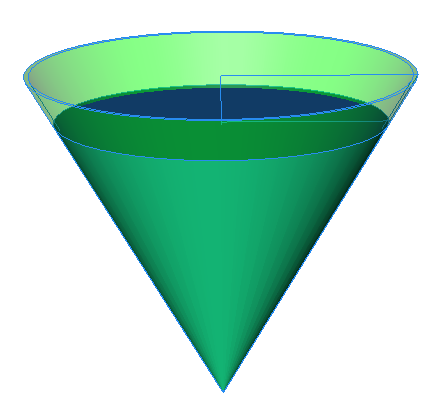
\includegraphics[width=2in]{img/filled_cone.png} }}%
        \qquad\qquad
        \subfloat[side view]{{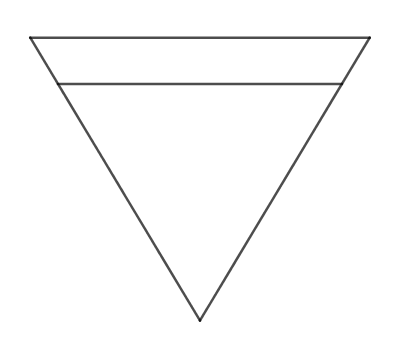
\includegraphics[width=2in]{img/filled_cone_diagram.png} }}%
        % \caption{2 Figures side by side}%
        \label{fig:example}%
       \end{figure}
\end{enumerate}




\end{document}
